The HPS Test Run was proposed to DOE early in 2011 as the first stage of the HPS experiment. Its
purposes included demonstrating that the apparatus and data acquisition systems would work well,
that the trigger rates and occupancies to be encountered in electron-beam running were as simulated,
and that the apparatus would performed as needed to conduct the HPS experiment. It would also
provide valuable experience to the HPS Collaboration in all aspects of designing, building, installing,
and running the experiment at JAB. It was hoped that the experiment would get dedicated run time
in an electron beam and even, if things performed as expected, that HPS could begin its search for
heavy photons. The HPS Test Run was installed on April 19, 2012, and ran parasitically with the HDice
experiment, using a photon beam, until May 18. The JLAB run schedule precluded any dedicated
electron beam running, but the HPS Test Run did get some valuable dedicated photon beam running.

This section briefly reviews the HPS Test Run apparatus, which is a simplified version of the apparatus
described above for the full HPS experiment, and demonstrates the feasibility of the detector
technologies proposed for silicon tracker, ECal, and data acquisition systems. It documents the
performance of the trigger, data acquisition, silicon vertex tracker, and electromagnetic calorimeter
and shows that the performance assumed in calculating the physics reach of the experiment is realistic.
Of particular importance, data from the dedicated photon beam running has been used to compare
the observed trigger rates with that expected in simulation. The trigger rate is almost entirely due to
photons which have converted to e$^+$e$^-$ upstream of the HPS trackers, and is sensitive to the multiple
Coulomb scattering of the electrons in the conversion target. Good agreement between data and
simulation confirm the EGS5 simulation and its description of multiple Coulomb scattering. Since
multiple Coulomb scattering of the electron beam dominates the SVT occupancies and ECal trigger rates
in HPS, confirming the simulation has demonstrated that backgrounds in HPS are understood.

In addition to the important test of our simulation tools, the HPS parasitic tests, staged over the Hall-B HDice run (g14), accomplished the following: 
\begin{enumerate}
\item  integrated SLAC and JLAB readout systems into a single DAQ
\item fully tested the Level 1 trigger system based on FADCs
\item tested experimental monitoring and controls
\item gained experience with running the test apparatus, in particular running SVT in vacuum
\end{enumerate}

\subsection{HPS Test Run Apparatus } 

In Figure \ref{fig:hpstest_layout}, the layout of the parasitic run is shown. The silicon vertex tracker was installed inside the Hall B pair spectrometer magnet vacuum chamber. The electromagnetic calorimeter was mounted downstream of it.
Both the Si-tracker and the ECal were retracted off the beam plane to allow clean passage of the photon beam through the system, and also not to obscure converted (e$^+$e$^-$) pairs from being detected in the PS hodoscopes.
 
\begin{figure}[ht]
    \includegraphics[width=\textwidth]{test2012/HPS_dimensions}
\caption{\small{Layout of the HPS parasitic run.} }
\label{fig:hpstest_layout}
\end{figure}

For the portion of the dedicated HPS run the photon beam was generated in the interaction of the $5.5$ GeV electrons with a gold radiator of $10^{-4}$ r.l., located $\approx 8$ meters upstream of the PS pair converter. After collimation ($D=6.4$ mm), the photon beam passes through the pair converter and through the HPS system. Data were taken on different converters (empty, $1.8\times 10^{-3}$ r.l., $4.5\times 10^{-3}$ r.l., and $1.6\times 10^{-2}$ r.l.). These measurements were repeated for reverse field setting of the pair spectrometer dipole.


\subsubsection{Test Run SVT}

The silicon tracking and vertexing detector for HPS Test, or SVT, operates in an existing vacuum chamber inside the pair spectrometer analyzing magnet in Hall B at JLab.  The design principles of the SVT are described in further detail in the HPS Test Run Proposal  \cite{HPS_tPROP}. There are five measurement stations, or ``layers,'' placed immediately downstream of the target. Each layer comprises a pair of closely-spaced planes and each plane is responsible for measuring a single coordinate, or ``view.'' Introduction of a stereo angle between the two planes of each layer provides three-dimensional tracking and vertexing throughout the acceptance of the detector with one redundant layer. 

In order to accommodate the dead zone, the SVT is built in two halves that are mirror reflections of one another about the plane of the nominal electron beam.  Each half consists of five double-sided modules mounted on a support plate that provides services to the modules and allows them to be moved as a group relative to the dead zone. Each module places a pair of silicon microstrip sensors back-to-back at a specified stereo angle with independent cooling and support.

100 milliradian stereo is used in the first three layers to provide higher-resolution 3-d space points for vertexing. The 50 milliradian stereo of the last two layers breaks the tracking degeneracy of having five identical layers and minimizes fakes from ghost hits, improving pattern recognition while still providing sufficient pointing resolution into Layer 3 for robust hit association in the denser environment there. These stereo angles are the same as those proposed in Section \ref{sec:svtt} for the new SVT. The details of the five layers are shown in Table \ref{tab:trk} and a solid model of the detector layout is shown in Figure \ref{fig:tracker_model}.  Figure \ref{fig:tracker_halves} shows a photograph of both completed detector halves prior to final assembly.  Altogether, this layout comprises 20 sensors and hybrids and 100 APV25 chips for a total of 12780 readout channels. 

\begin{table}[h]
\begin{center}
\begin{tabular}{lccccc}   
\hline \hline 
    Layer & 1 & 2 & 3 & 4 & 5 \\      
\hline
    nominal $z$, from target (cm)  & 10 & 20 & 30 & 50 & 70  \\ 
    Stereo Angle (mrad)  & 100 & 100 & 100 & 50 & 50 \\ 
    Bend plane resolution ($\mu m$)  & $\approx$6 & $\approx$6 & $\approx$6 & $\approx$120 & $\approx$120  \\ 
    Non-bend plane Resolution ($\mu m$)  & $\approx$6 & $\approx$6 & $\approx$6 & $\approx$6 & $\approx$6  \\ 
    \# sensors  & 4 & 4 & 4 & 4 & 4  \\ 
    Nominal dead zone  & $\pm1.5$  & $\pm3.0$  & $\pm4.5$  & $\pm7.5$  & $\pm10.5$  \\ 
    Power consumption & 6.9 & 6.9 & 6.9 & 6.9 & 6.9 \\
\hline \hline
\end{tabular}
\caption[]{Layout of the HPS SVT. }
\label{tab:trk} 
\end{center}
\end{table}

\begin{figure}[ht]
    \includegraphics[width=\textwidth]{test2012/HPS_nocables_nowires}
\caption{\small{A partial rendering of the HPS Test SVT solid model showing the modules of the upper and lower half-detectors on their support plates, the hinged C-support, the motion levers, the cooling manifolds on their strain relief plate and the baseplate with its adjusters.  The sensors are shown in red and the hybrids in green. The beam enters from the right.} }
\label{fig:tracker_model}
\end{figure}

\begin{figure}[ht]
    \includegraphics[width=\textwidth]{test2012/2012-101-PHOTON-DETECTOR-001.jpg}
\caption{\small{Both halves of the HPS Test SVT fully assembled at SLAC.} }
\label{fig:tracker_halves}
\end{figure}

Power is provided to each hybrid using CAEN power supplies provided by Fermilab. Three low voltages are supplied for the APV25 and one high voltage to reverse bias the sensor. The supplies that provide sensor bias are capable of 500V operation and can be used to test operation at high voltage in close proximity to an electron beam. The total power consumption of each hybrid during normal operation is about 2 W, which is removed with the cooling system. Care was exercised in selecting power and data cables, to ensure vacuum compatibility and sufficient radiation hardness. The teflon-coated twisted pair copper wires selected are rated for 400kRad, well above the expected exposure of 20kRad/week. A special purpose junction box interfaces the CAEN power supply output channels to the SVT hybrids. Control of the supplies is provided via an EPICS graphical user interface, which allows monitoring of the detector and interlock protection as well.

The linear shifts that define the opening of the SVT are controlled by a pair of stepper motors located in low field regions at the ends of the analyzing magnet.  For photon running, these are locked in the open position, but for electron running they will be connected and controlled through EPICS so that the distance between the beam and the sensors can be adjusted to balance detector occupancies and acceptance.


\subsubsection{Test run ECal}

The HPS Test Run electromagnetic calorimeter (ECal) consists of 442 lead-tungstate (PbWO$_4$) crystals with avalanche photodiode (APD) readout, \cite{HPS_PROP_UPD}. 
Crystals in the ECal are arranged in two modules.  There are 5 layers in each module;  four layers have 46 crystals and one has 37.  The ECal is mounted downstream of the analyzing dipole magnet at the distance of $\sim 148$ cm from the upstream edge of the magnet. The two ECal modules are positioned just above and below the beam plane such that the edge of the crystal closest to the beam is $3.7$ cm from it. As was described in Section \ref{setup} we did not use the vacuum chamber between the two ECal modules for the photon test run, instead 2'' beam pipe was used to transport photon beam from the pair spectrometer vacuum chamber to HDIce target.  

\begin{figure*}[t]
\includegraphics[ scale=0.25]{test2012/ecal_assembly.jpg}
\caption{\small{Assembly of the ECal bottom module.}}\label{fig:ecal_assembly}
\end{figure*}

In order to maintain stable performance of the PbWO$_4$ calorimeter, the crystals and APDs are enclosed within a temperature stabilized environment, held constant at the level of $1~^o$F. The expected energy resolution of the system from operational experience with the IC is $\sigma_E/E \sim 4.5\% / \sqrt{E (GeV)}$. As in the IC, PbWO$_4$ modules are connected to a motherboard that provides power to and transmits signals from individual APDs and pre-amplifier boards. Crystals inside the box are supported by aluminum frames, Figure \ref{fig:ecal_assembly}.

For this run the ECal made use of the existing low and high voltage systems from the CLAS/IC, as well as signal cables and splitters. Connectors on the existing signal cables have been rearranged to accommodate the new layout of the channels. 
 
In Figure \ref{fig:ecal_mounted} ECal is shown in its installed position for the parasitic run with photon beams. It centered relative to the beam that passes in between two parts of ECal through $3$ inch beam pipe. Cooling lines, as well as signal, HV and LV cables are visible. 
 
\begin{figure*}[t]
\includegraphics[ scale=0.25]{test2012/ecal_mounted}
\caption{\small{ECal mounted downstream of the Hall-B pair spectrometer for the parasitic run with photon beams. Hoses for the cooling system, and the power and signal cables for beam-right side of both modules are visible.}}\label{fig:ecal_mounted}
\end{figure*}



\subsubsection{Test Run Data Acquisition}
\label{sec:testrun_daq}
The test run served as a proof of principle for the proposed DAQ and the system was very 
close to that proposed for HPS. Since the systems are similar only the main differences will be highlighted here,  with more details in Section~\ref{sec:daq} and with results and experiences discussed below in Section~\ref{sec:testrun_performance}. 


A generic layout of the hardware from the test run DAQ is laid out in Figure~\ref{fig:daq}.
 \begin{figure*}[h]
\includegraphics[scale=0.35]{test2012/daq/daq_schem.pdf}
\caption{\small{Readout and processing system block diagram.}}\label{fig:daq}
\end{figure*}
The front-end systems of the ECal and SVT are similar. 
The differences of the DAQ and trigger w.r.t. to the HPS are fleshed out in greater detail below but 
are all related to the following areas:
\begin{enumerate}
\item a lower ECal cluster resolution and no calibration available at the trigger level together with simpler trigger logic, 
\item a smaller SVT without the need for optical readout and power distribution inside the vacuum,
and
\item lower bandwidth links.
\end{enumerate}

The two front-end electronics systems for the ECal and SVT are essentially unchanged. The ECal provides 
input to the Level~1 trigger system after which an accepted event is acquired from the two sub-systems 
and are processed in the data acquisition and processing system. The Readout Crate Controllers (ROCs)
 described for HPS are unchanged and installed in every VME, VME64X, VXS crates running 
 mvme6100 controllers with a prpmc880 or pmc280 co-processor modules. A hybrid approach was 
 used for the SVT DAQ in the test run where the ROC ran on a external PC connected to the ATCA crate. 
 Similar to HPS, a Foundry Router was used as the backbone of the DAQ system, providing 1Gbps and 
 10Gbps connections between components and to the JLAB Computer Center.

The Event Builder, Event Recorder, and other critical DAQ components ran on 
4-CPU Opteron-based servers, which was sufficient for the test run. The RAID5 test run storage system 
had a 100~MByte/sec capability which was well enough for the data rates attained in the test run as 
described below. 

%\subsubsection{SVT DAQ}



The SVT DAQ was a rapidly built DAQ  designed to readout data continuously at 40 MHz from the silicon detector modules, and transfer data to the JLab DAQ once a trigger signal is received. It is built using the same 
basic architecture and layout as the HPS DAQ but without the optical readout components and 
power distribution system inside the vacuum described in Sec.~\ref{sec:svt_daq}. 

The test run had a total of 20 silicon strip sensors, each one connected to an onboard hybrid readout card 
which is similar to the HPS hybrid, each one holding five 128-channel APV25 integrated circuits. The test 
run hybrid readout card is shown in Fig.~\ref{fig:hybrid_and_apv25_testrun} 
 \begin{figure*}[t]
\includegraphics[ scale=0.3]{test2012/daq/hybrid.jpg}
\includegraphics[ scale=0.3]{test2012/daq/apvs-on-hybrid.jpg}
\caption{\small{Picture of a test run hybrid readout board holding five APV25 ASICs. The wire bonds to the 
silicon sensors can be seen as well.}}
\label{fig:hybrid_and_apv25_testrun}
\end{figure*}

Contrary to the HPS DAQ where opto-boards digitizes and converts the APV25 analog output signals to 
optical signals inside the vacuum chamber, the hybrids here carry analog signal directly to the 
Rear Transistion Module (RTM) via a multi-twisted-pair cable. The amplification and digitization of the 
analog differential voltage output of the APV25 output are therefore carried out on the RTM board 
which was designed specifically for the HPS test run. Figure~\ref{fig:svtdaq} shows an overall layout of 
the SVT test run DAQ system (compare to Fig.~\ref{fig:svt_daq_overview}).
 \begin{figure}[t]
\includegraphics[scale=0.9]{test2012/daq/svt_daq_diagram.png}
\caption{\small{Schematic of the SVT DAQ showing input from the hybrids mounted on the silicon detector to the RTM, its connection to the COB, and the Ethernet switch used to transfer data at 1 Gbps to the 
DAQ PC and ultimately to the JLAB DAQ.}}
\label{fig:svtdaq}
\end{figure}
On the RTM, a pre-amplifier converts the APV25 differential current output to a different voltage output 
scaled to the sensitive range of a 14-bit ADC. The RTM is organized into four sections with each section 
supporting 3 hybrids (15 channels). 
The ADC is operated at the system clock of 41.667 Mhz. 
%The RTM also includes a 4-channel Fiber Optic module and supporting logic which can be used to interface to the JLAB trigger supervisor card.
The ATCA main board (the Cluster On Board or COB) is similar to the HPS DAQ with the important exception that one of the DPM's functions as the trigger interface only and there is no RCE module. 
Instead, the DPMs package and send the data from the hybrids to an external PC through a 1Gbps 
ethernet connection which serve the same purpose as the RCE module in the HPS DAQ. 
The ATCA crate hosts two COB cards, one supporting four data processing DPMs and the other supporting three data processing DPMs and one trigger DPM to support a total of 21 hybrids, one more than required. 
The test run RTM and COB can be seen in Fig.~\ref{fig:rtm_testrun}. 
\begin{figure*}[t]
\includegraphics[ scale=0.25]{test2012/daq/rtm.png}
\includegraphics[ scale=0.4]{test2012/daq/svt_daq_module_noted.png}
\caption{\small{Picture of a RTM (top) and COB board (bottom) used in the HPS test run 2012.}}
\label{fig:rtm_testrun}
\end{figure*}
The external PC supports three network interfaces, 2 standard 1G-bit Ethernet and one custom low latency data reception card. The first Ethernet interface is used for slow control and monitoring of the 8 DPM modules. The second Ethernet interface serves as the interface to the JLAB data acquisition system. The third custom low latency network interface is used to receive data from the SVT ATCA crate and supports a low latency, reliable TTL trigger acknowledge interface to the trigger DPM. This PC hosts the SVT control and monitoring software as well as the JLAB ROC (Read Out Controller) application.


The ECal DAQ system used in the test run is very similar to that described for HPS in Sec.~\ref{sec:fadc_daq}. 
The only significant difference is that in the test run, the signals from the ECal modules were sent to a signal splitter. One of the outputs of the splitter is fed to a 
discriminator that also has an internal scaler, and then to a TDC channel. The other output is sent to the 
JLab FADC250 VXS module, shown in Fig.~\ref{fig:fadc}.
%, is based on information from the FADC boards and includes a cluster 
%finding algorithm using FPGA modules. With the FADC-based system, the energy of clusters used to 
%make a trigger decision is determined at the crate level. 






\subsubsection{Test Run Trigger System}
\label{sec:testrun_trigger}

A block diagram of the HPS test run trigger processing is shown in Fig.~\ref{fig:trigger_diagram}.  A gigabit bandwidth is used to transport all the individual FADC250 channel sums (5-bits) and clock (3-bits) encoding bits to resolve a $4$~ns period within a $32$~ns frame.  The clock encoding bits report the time when the input signal crosses the programmable threshold within the $32$~ns frame.  If the input signal does not cross threshold for a given $32$~ns frame, then the channel data is reported as zero.
\begin{figure}[t]
\includegraphics[scale=0.6]{test2012/trigger/HPSChanSum_001.jpg}
\caption{\small{Block diagram for the trigger system.}}\label{fig:trigger_diagram}
\end{figure}

The reported 5-bit channel sum value is extracted from the 17-bit register that contains the integrated (sum) signal value of the input channel.  The channel integration occurs only if the input signal crosses the programmable threshold level.  The samples that are included in the channel integration are those that are above threshold.  The number of samples for a given channel integration will not be larger than the frame report latency time (128~ns or 32 samples). Samples of the input signal are shown in Fig.~\ref{fig:trigsamples}. The point where the input signal crosses threshold determines which frame the integrated value is reported.  The time where the input signal crosses threshold is captured within the frame and reported with the three clock encoding bits to a 4~ns time stamp of the threshold crossing time.
\begin{figure}[t]
\includegraphics[scale=0.9]{test2012/trigger//trigger_pulse_samples}
\caption{\small{Example of input signals, and how they are integrated for the test run trigger.}}\label{fig:trigsamples}
\end{figure}
In the example, the pulse for channel~2 crosses multiple frames.  The point where the signal crosses threshold determines the frame where the integration value will be reported for the given channel.  The number of points that are above threshold will be limited to 32. If multiple pulses arrive within a 32~ns frame, they will not be resolved and thus create a pile-up effect.  The trigger application will only process a single falling edge or single rising edge per 32~ns frame. Multiple pulses per frame can be recovered from the readout data offline.

Information from each FADC channel were reported to the Crate Trigger Processor (CTP) through Gigabit serial data streams. The sixteen serial data streams will be processed on a frame by frame basis, and the cluster finding algorithm (same as for HPS in Sec.~\ref{sec:triggerdaq}) will produce a serial data stream that will be processed by the Sub-System Processor (SSP) to create a readout trigger signal that can be distributed to the front end FADC250 for Physics event readout. The system was designed for maximum trigger accept rate of 50~kHz. 

For the test run, the trigger decision in the SSP was a simple threshold: the trigger would fire on a single cluster with energy exceeding the threshold. The full trigger described in \cite{HPS_tPROP} was however implemented and tested.






\subsection{Test Run Apparatus Performance} 
\label{sec:testrun_performance}
As noted above we only had the opportunity to tun the HPS test apparatus in the 
photon beam mode using the Hall-B pair 
spectrometer (PS) pair converter as a target, which is located $\sim 67$ cm from the first layer 
of the tracker. This section will report on a few selected preliminary results that aims to demonstrate 
our understanding of the main characteristics of the system. 

\subsubsection{SVT Performance}
\vspace{1cm}{\bf Calibration [Omar]}


Description of hit amplitude, baseline/gain calibration, noisy channels/chips, pulse shape cuts, occupancy. 

Plots: Response plot, gain, noisy channels vs run nr?, data/MC of noise hits,Data/MC plot of occupancy for some layers  

\vspace{1cm}{\bf Cluster reconstruction [Omar]}


Description of the cluster reconstruction.

Plots: mip distribution

\vspace{1cm}{\bf SVT timing [Sho]}

The time reconstruction algorithm described in \ref{sec:svtŧ} was used to fit a single hit to each SVT channel in each event.
Pileup was not considered due to the very low hit rate in the SVT.

Values of fit $\chi^2$ fell in the distribution of $\chi^2$ for 4 degrees of freedom (6 points -- 2 fit parameters), as expected.

After clustering these hits, the hit time for the cluster is computed as the amplitude-weighted average of the channel hit times. 

Description of the SVT hit time reconstruction. 

Plots: example time fits, mean hit times across tracker, plot of simulated time resolution vs S/N? 

\vspace{1cm}{\bf Tracking algorithms [Matt/Omar]}


Pattern recognition/Stereo hit reconstruction and description of the tracking algorithm. 

 Plots: tracking efficiency vs run nr, hit efficiency vs run nr for data. Overlay MC.
 
\vspace{1cm}{\bf Tracking algorithms [Matt]}


Analysis of two track events. 

Plots: invariant mass, vertex position, 2-track event multiplicity. Compare with MC for all these 

\label{sec:svtperformance}

%Good alignment of the SVT is critical to achieving the expected tracking performance and physics reach. 
%The sensors must be aligned internally and with respect to the target and other beam line components for optimal performance. 
%The alignment of the test run apparatus proceeds in several steps which must be tied together to achieve the final alignment.
%These include survey measurements of various SVT assemblies, a beam line survey at JLab, and finally 
%a track-based alignment. 

The SVT was aligned using a combination of optical, laser and touch probe surveys at SLAC and JLab. The 
optical survey of individual modules with precision of a few microns are combined with a touch-prove survey 
of the overall SVT support structure, with 25-100 microns precision, to locate the silicon sensor layers with 
respect to the support plates and the mechanical survey balls on the base plate.
%Mechanical surveys using touch probes was performed on the two SVT tracker planes before 
%shipping to JLab. This survey measured reference points on the base plate, C-support and on the surface of the tracker support plates. These positions where then tied to very precise optical survey of each sensor module, referencing the silicon sensor position w.r.t. to the cooling blocks. 
%An important aspect of the mechanical survey is the relatively large sag of 
%the 70~cm long support plate which is supported by the C-support hinge on one end and the 
%extension bar attached to the linear shaft at the other. The measured sag without all services 
%(cooling manifold and cables was not dressed at this point) was more than $250~\mu$m.  
%For HPS, only the first three layers are being supported from each end which will reduce this 
%sag with at least a factor of four. {\color{red} check this}. The goal of the mechanical surveys is 
%to reach a relative alignment of the 
%silicon to about $100-200~\mu$m where alignment using tracks become feasible and the 
%improvements from mechanical surveys become harder. 
After full assembly and installation of the SVT at JLab, a mechanical survey of the SVT base plate position 
inside the pair spectrometer vacuum chamber is used to determine the global position of the SVT with respect 
to CEBAF beam line. 
%at the as-built alignment.  The sag
%of the long support plates and lever arms used in the test run are the dominant error in determining
%relative modules positions, a defect addressed in the proposed design for the SVT.
%Finally at JLab, with a fully assembled 
%tracker, an optical and touch probe survey was performed to locate 
%the SVT inside the vacuum chamber, using the measurements of the base plate, in the reference coordinate system of 
%the analyzing magnet. 
The resulting survey-based alignment has the position of the silicon sensors correct to within a few hundred 
microns as shown in the mean of the biased track residuals in Fig.~\ref{fig:res_top}.  The large multiple scattering contribution can be seen by the large increase in the width of the residuals in the later layers. The agreement with simulation is reasonable; a slight track reconstruction algorithm bias can be seen in the mean for the simulation in later layers which will be fixed in the future. 
%This level of internal alignment 
%shows that the survey approach, while not perfect, is adequate as a starting point to bootstrap the SVT 
%alignment. 
%At this level of internal 
%alignment   an internal SVT alignment with track residuals less than a few 
%hundred microns shown in .  is then studied using reconstructed tracks in the SVT. The main observable of the internal alignment of the silicon 
%sensors is the so-called track residual. It is 
%defined as the difference of the measured and predicted track 
%position at that sensor. Figure~\ref{fig:res_top} 
%shows representable 3D space point track residuals, relative to track parameters determined at the target, for tracks reconstructed in the top half of the tracker.
\begin{figure*}[]
\includegraphics[ scale=0.3]{test2012/alignment/pictures/res_top/h_trk_top_res_y_mean_h_trk_top_res_y_mean_dataMC_trigseltwotrksel4hit_recoilmc_twotrkfilt.png}
\includegraphics[ scale=0.3]{test2012/alignment/pictures/res_top/h_trk_top_res_z_mean_h_trk_top_res_z_mean_dataMC_trigseltwotrksel4hit_recoilmc_twotrkfilt.png}
\includegraphics[ scale=0.3]{test2012/alignment/pictures/res_top/h_trk_top_res_y_sigma_h_trk_top_res_y_sigma_dataMC_trigseltwotrksel4hit_recoilmc_twotrkfilt.png}
\includegraphics[ scale=0.3]{test2012/alignment/pictures/res_top/h_trk_top_res_z_sigma_h_trk_top_res_z_sigma_dataMC_trigseltwotrksel4hit_recoilmc_twotrkfilt.png}
\caption{\small{Mean (top) and standard deviation (bottom) of biased residuals (i.e. hits are included in the track fit) between the actual hit position and the predicted position from the reconstructed tracks in the bend (left) and non-bend (right) plane in the top half of the SVT after mechanical survey. The smaller width for the 5th layer in the bend plane is an effect from mixing tracks with four or five hit tracks.}}
\label{fig:res_top}
\end{figure*}
%These are compared to the residuals from an ideally aligned tracker with residuals centered at zero.
%Note the larger width for the downstream layers,highlighting the large 
%multiple scattering contribution in the track reconstruction. 
%The intrinsic single hit resolution of $\approx 6~\mu$m is negligible for layers beyond the second. 
%Fig.~\ref{fig:res_top_summary} shows a summary of the mean residuals for each layer of the tracker 
%after the mechanical survey alignment constants have been applied.
%\begin{figure*}[t]
%\includegraphics[ scale=0.7]{test2012/alignment/pictures/res_top/res_top_summary-1.png}
%\includegraphics[ scale=0.7]{test2012/alignment/pictures/res_top/res_top_summary-2.png}\caption{\small{Mean of the track residuals for each detector layer in the top tracker half 
%in the bend (left) and non-bend (right) plane after mechanical survey constants are applied.}}\label{fig:res_top_summary}
%\end{figure*}
%Note that these pull distributions come from biased 
%residuals (the hit was used in the track fit) and are thus not expected to have a 
%width of one. 
%\begin{figure*}[]
%\includegraphics[ scale=1.2]{test2012/alignment/pictures/res_pull_top/res_pull_top-1.png}
%\includegraphics[ scale=0.5]{test2012/alignment/pictures/res_pull_top/res_pull_top-2.png}
%\includegraphics[ scale=0.5]{test2012/alignment/pictures/res_pull_top/res_pull_top-3.png}
%\includegraphics[ scale=1.2]{test2012/alignment/pictures/res_pull_top/res_pull_top-4.png}
%\includegraphics[ scale=0.5]{test2012/alignment/pictures/res_pull_top/res_pull_top-5.png}
%\includegraphics[ scale=1.2]{test2012/alignment/pictures/res_pull_top/res_pull_top-6.png}
%\includegraphics[ scale=0.5]{test2012/alignment/pictures/res_pull_top/res_pull_top-7.png}
%\includegraphics[ scale=0.5]{test2012/alignment/pictures/res_pull_top/res_pull_top-8.png}
%\includegraphics[ scale=1.2]{test2012/alignment/pictures/res_pull_top/res_pull_top-9.png}
%\includegraphics[ scale=0.5]{test2012/alignment/pictures/res_pull_top/res_pull_top-10.png}
%\caption{\small{Track residual pulls in the bend (top) and non-bend (bottom) plane 
%for tracks reconstructed in the 
%top half of the tracker.  }}
%\label{fig:res_pull_top_nonbend}
%\end{figure*}

%In electron running, the beam spot can be used as a constraint in the global track-based alignment. 
We also extrapolate the reconstructed tracks back to the converter located $\approx 77$~cm 
from our first silicon layer to understand the tracker alignment w.r.t. to the other components on the 
beam line. Figure~\ref{fig:extrapol_converter} shows good agreement of the reconstructed track position at the converter with that predicted from simulation using the measured field map of the analyzing magnet to take into account the fringe field. The offset of the horizontal position simply reflects the fact that the positions are reconstructed in an SVT-centered coordinate system, which is tilted with respect to the beam coordinate system.
\begin{figure*}[t]
\includegraphics[ scale=0.25]{test2012/alignment/pictures/extrapolation_converter/h_trk_top_fr_conv_y_h_trk_top_conv_y_dataMC_twotrksel.png}
\includegraphics[ scale=0.25]{test2012/alignment/pictures/extrapolation_converter/h_trk_top_fr_conv_z_h_trk_top_conv_z_dataMC_twotrksel.png}
%\includegraphics[ scale=0.5]{test2012/alignment/pictures/extrapolation_converter/extrapolation_Y_converter_top.png}
%\includegraphics[ scale=0.5]{test2012/alignment/pictures/extrapolation_converter/extrapolation_Y_converter_bot.png}
\caption{\small{Extrapolated track positions for reconstructed e$^{+}$e$^{-}$ pairs in the SVT taking into account the measured fringe field of the analyzing magnet. 
The filled histograms show the prediction from simulation using an ideal geometry. 
A shift in the bend-plane coordinate for tracks in the bottom half (top right) is likely due to alignment or incomplete description of the
magnetic field at the edge of the magnet.
%The extra bumps in the data at $\pm10$~mm arise from backgrounds originating upstream of the 
converter.
}}
\label{fig:extrapol_converter}
\end{figure*}
%The width is roughly consistent with between data and simulation with a shift in the bend-plane 
%coordinate for tracks in the bottom half which is likely due to alignment or incomplete description of the 
%magnetic field at the edge of the magnet. 
%There are two small bumps in the vertical position in the data arising from backgrounds 
%originating upstream of the converter verified using the run without a converter.
%The luminous region, inferred from harp scans of the photon beam profile, has a width of about 1~mm 
%%(best described by a double Gaussian: $0.71e^{\frac{x}{0.366}}\times 0.29e^{\frac{x}{1.111}}$)
%and a total beam envelope of around 7~mm. The small bumps in data at $\pm10$~mm 
%are from particles produced upstream of the converter. The width and position of the tracks 
%are roughly consistent with the expected distribution from an ideal geometry as shown by the simulated 
%tracks in the same figures. The larger shift in the bend direction for bottom tracks 
%is still under investigation. 

With initial residuals less than $\sim 500~\mu$m across all layers of 
the tracker and a reconstructed beam profile similar to that expected from simulation, it appears these survey techniques 
are adequate to bootstrap the SVT alignment. 
For HPS, we are developing a more sophisticated global track-based alignment technique to reach 
the final alignment precision. This framework will also enable us to explore and understand important details 
such as weak modes and how dedicated alignment runs 
(e.g. with magnetic field off or with different targets) may shape operational procedures during HPS running.
%Fig.~\ref{fig:test_harpscan} shows a HARP scan taken during the test run. 
%\begin{figure*}[t]
%\includegraphics[ scale=0.5]{test2012/alignment/pictures/harp_scan_testrun.png}
%\caption{\small{Photon beam profile HARP scan close to the converter.}}\label{fig:testrun_harpscan}
%\end{figure*}
%The width of the beam can be described by a double Gaussian $0.71e^{\frac{x}{0.366}}\times 0.29e^{1.111}$ which is also used in the simulations. The beam envelope extends out to 
%about 7mm. 


\subsubsection{ECal \& Trigger Performance}

\vspace{1cm}{\bf ECal performance [Sho]}

The ECal preamplifiers shape the APD signal into a CR-RC pulse of rise time $\approx 14$ ns; this is sampled every 4 ns and stored in a pipeline on the FADC readout board.
On receiving a trigger, the FADC searches for rising threshold crossings in the pipeline, and integrates pulses by summing 5 samples before and 30 samples after each threshold crossing.

The noise and pedestal of the readout chain are calibrated by running the

Of 442 crystals/channels, 39 were disabled or disconnected and were not read out by the DAQ. 
13 of these were not read out because of a shortage of FADC readout boards.
The remainder either had no HV bias on the APD, or were disabled in the FADC software due to noise.

In the data, we identified two types of abnormal channels. 
One FADC was not sending trigger signals correctly, resulting in low efficiency. This affected the 13 channels read out by that FADC.
5 channels were diagnosed as noisy because they had a high incidence of hits out of coincidence with the trigger.

A large number of channels were originally misidentified as noisy because they had much higher hit occupancy than neighboring channels.
Gain calibration (described in the next section) shows that these channels have high gain (and thus lower energy threshold) but are otherwise normal.

The abnormal channels were ignored in analysis in order to simplify comparison with Monte Carlo. This leaves 385 useful channels---87\% of the ECal.

We found that one quadrant of the ECal had been miswired in such a way as to flip the horizontal coordinate---the column of crystals nearest the center was connected to the readout channels for the rightmost column, and vice versa.


Describe clustering, thresholds, occupancy, dead/noisy crystals, flip in readout?

Plots: Occupancy map

\begin{figure}[ht]
	\includegraphics[width=0.5\textwidth]{test2012/ecalperformance/hitrates}
	\caption{\small{}}
	\label{fig:hitrates}
\end{figure}

\vspace{1cm}{\bf ECal Calibration [Sho]}


Description of the gain calibration. Relate to how good it needs to be which should be in the performance section. Discussion of sampling fraction. Relation to what calibration that is needed for the trigger in 2014?

Plots: E/p map before and after calibration, spread in gain, E/p data/MC


\vspace{1cm}{\bf Trigger performance [Sho/Ben]}

%\begin{figure}[ht]
%	\includegraphics[width=\textwidth]{test2012/ecalperformance/trigtimes}
%	\caption{\small{}}
%	\label{fig:trigtimes}
%\end{figure}

As described in Section \ref{sec:tesrun_trigger}, the trigger and DAQ integrate pulses differently to measure hit energy. The trigger integrates using a time-over-threshold window, and the DAQ readout integrates using a constant window (5 samples before and 30 samples after a threshold crossing). 

For every event, the trigger reports as a bitmask the trigger decision (top trigger, bottom trigger, or both) and the time the trigger fires.

We study trigger performance by simulating the trigger for each event and comparing actual To study trigger performance, we first convert from readout hits (constant integration window) to trigger hits (time-over-threshold integration). 
This is done by converting from the readout hit to pulse amplitude, then applying the time-over-threshold algorithm to the simulated ECal pulse shape. 
We then simulate the CTP clustering algorithm and the trigger decision, and compare the trigger decision and trigger time reported by the simulation to what was reported by the real trigger.

To eliminate trigger bias in checking the trigger decision, we use a tag and probe method: to check trigger performance in one half of the ECal, we tag events where there was a trigger in the other half, and exactly one probe cluster in the ECal half under test. 
We then measured trigger efficiency (proportion of tagged events where there was a trigger) as a function of ADC counts and energy of the probe cluster.

These turn-on curves are shown for the top half of the ECal in Figure \ref{fig:turnon}. 
The trigger threshold is seen to be 1280 ADC counts as expected; the threshold is not perfectly sharp in this analysis because of uncertainties in the conversion from constant-window to time-over-threshold integrals, but based on comparisons with Monte Carlo simulation we believe the trigger worked exactly as specified. 
The trigger threshold in terms of cluster energy is very uneven for two reasons: gain variations between different ECal crystals lead to threshold variations, and the nonlinearity of the time-over-threshold integral means that the effective threshold is higher for clusters that span multiple crystals.

\begin{figure}[ht]
	\includegraphics[width=0.4\textwidth]{test2012/ecalperformance/top_turnon_adc}
	\includegraphics[width=0.4\textwidth]{test2012/ecalperformance/top_turnon_e}
	\caption{\small{Trigger turn-on as a function of probe cluster ADC counts (left) and probe cluster energy in MeV (right). Both plots are for the top half of the ECal; bottom is similar. 
	Energy is not corrected for sampling fraction.}}
	\label{fig:turnon}
\end{figure}

Overall the trigger appears to have functioned exactly as intended. Changes planned for the next run (constant integration window and per-crystal gain calibration constants for the trigger) will solve both of the issues that led to threshold variations in the test run.

What were the rates, lessons learned?

Plots: Compare observed and expected trigger time {\it Sho}, Tag\&probe {\it Sho}, rates vs time {\it Ben/Sho/Pelle}



\label{sec:ecalperformance}

\subsubsection{Multiple Coulomb Scattering Measurement}
\label{sec:angular_measurement}

One of the main parameters that has the 
largest impact on the main design of the HPS experiment is the occupancies expected 
close to the beam.  The largest contribution comes from electrons scattered to large angles 
in the target. It is worth remembering that HPS is sensitive to scattering angles very far out 
on the tail which has been less explored in past experiments. One of the main goals of the 
test run in 2012 was to evaluate the description of the tails of the multiple scattering in order 
to gain further confidence in our expected detector occupancy. As will be shown below, the 
test run was sensitive to the multiple coulomb scattering description despite the fact that 
the data was taken with a photon beam. The details of the test run conditions are described in Sec.~\ref{sec:testrun2012}. 

Figure~\ref{fig:schematic_testrun_vs_erun} gives a schematic view of the main differences 
between the photon and electron beam setup. 
\begin{figure*}[t]
\includegraphics[ scale=0.5]{test2012/angular_measurement/pictures/photon_vs_electron_beam_schematic.png}
\caption{\small{Schematic comparison of the photon beam setup to the electron beam.}}\label{fig:schematic_testrun_vs_erun}
\end{figure*}
In particular, the angular distribution of the pair produced electron and positions emerging 
from the target has contributions from two sources: {\it i} the pair production angle $\alpha$ 
and {\it ii} the resulting angle from multiple scattering in the target after production. This is 
schematically described in Fig.~\ref{fig:schematic_pair_prod}. 
\begin{figure*}[t]
\includegraphics[ scale=0.7]{test2012/angular_measurement/pictures/pair_prod_schematics.png}
\caption{\small{Schematic description of the relevant angles for pair production in the 
test run.}}\label{fig:schematic_pair_prod}
\end{figure*}
The contribution from both sources to the final angular distribution are comparable. FigureX 
shows the expected distribution of the vertical angle $\theta_y$ for the $e^+e^-$ pair  coming 
out of the converter compared to the pair production angle. {\color{red} Need this figure from Takashi.} 


{\bf Sample Composition}\newline
Since we are primarily interested in measuring the angular 
distributions for the $e^+e^-$ pair we checked that the contribution from photons are negligible. Table~\ref{tab:sample_composition} shows the sample composition. The fraction 
of photons that would deposit energy to reach threshold in the ECal crystals are much less than 2\% without any angular which will further reduce the fraction of photons. 
\begin{table}[]
\centering
\begin{tabular}{c|c|c|c}
Type & Nominal & $E>0.2$~GeV & $E>0.5$~GeV \\
\hline
electron & 7150 & 4938 & 3186 \\
positron & 6019 & 4568 & 2874 \\
$e^+e^-$ & 13169 & 9506 & 6060 \\
photon & 2984 & 640 & 151 \\
\hline
\end{tabular}
\caption{Sample composition for the photon test run. {\color{red} This needs to be updated 
or removed.}}
\label{tab:sample_composition}
\end{table}

The photon beam line during the test run presented a relatively large fraction of events 
originating upstream of the converter. This contribution was measured during data taking by 
removing the converter and thus taking data without any target but with all other conditions 
the same. Figure~\ref{fig:tracks_at_converter} shows the vertical position of 
reconstructed tracks in the SVT during data taking with the 1.6\% radiation length converter. 
Note the small satellite peaks visible at about $\pm 8$~mm. 
The same figure also overlays the same distribution for the empty converter 
run which clearly shows that these satellite peaks are due to the upstream backgrounds.
\begin{figure*}[t]
\includegraphics[ scale=0.6]{test2012/angular_measurement/pictures/tracks_at_converter_Y_top.png}
\includegraphics[ scale=0.6]{test2012/angular_measurement/pictures/tracks_at_converter_Y_bottom.png}
\caption{\small{Vertical position of extrapolated tracks from the SVT to the converter position.} {\color{red}Need update.}}\label{fig:tracks_at_converter}
\end{figure*}

In order to properly normalize the rates the integrated current was measured for the different 
runs. Typically the current was about 30~nA. Table.~\ref{tab:currents} shows the measured integrated currents. {\color{red} Describe how these where measured?}. The uncertainty 
of the measurement is estimated to approximately 5\%. 
\begin{table}
\centering
\begin{tabular}{l|c|c|c}
%Run & Target thickness [\%r.l.] &   start time[s]      & end time [s] & Duration [s] &       integrated beam current (nC)    \\                thickness (%r.l.)       Rate(Hz)     Recorded(Hz)  Magnet Polarity
Run & Target thickness & Duration &  $e^-$ on converter \\
 &  (\%r.l.) & (s) & (nC)    \\   
\hline\hline
1351 & 1.6   & 911 &     24385.9     \\
\hline
1353 & 0.18   & 2640 &    193508.9  \\
\hline
1354 & 0.45  & 2149 &       140709.9  \\
\hline
1358 & 0    & 1279  &   88079.6  \\
%1349    1337323714      1337324625      51344.0926551819        54879.7343788147        1.6                     1262.120     1174.728      -1
%1351    1337324962      1337325268      24385.9185791016        26928.0426635742        1.6                     1933.479     1696.808      -1
%1353    1337325717      1337328357      193508.881838322        204325.132622242        0.18                    436.895      425.659       -1
%1354    1337328521      1337330670      140709.898532331        148839.141475141        0.45                    596.055      570.870       -1
%1358    1337331152      1337332431      88079.5567516331        92523.9428218845        0                       309.785      304.253       -1
%1359    1337332615      1337334014      91653.0026320741        91761.4541434497        0                       318.640      311.540       1
%1360    1337334136      1337336898      198670.590789914        209883.979889035        0.18                    451.067      446.510       1
%1362    1337337264      1337338713      105642.70688653         110298.553449392        1.6                     1864.090     1659.675      1
%1363    1337340178      1337340456      8556.8459701538         8556.8459701538         1.6                     1864.090     1659.675      1
\hline
\end{tabular}
\caption{{\small Measured integrated currents for the runs used to measure the angular distributions.}}
\end{table}
Taking into account the luminosity the upstream background fraction was 16\%, 52\% and 71\% 
for converter thickness of 1.6\%, 0.45\% and 0.18\%, respectively. 

The measured angular distribution in the ECal for the three target thicknesses are shown in 
Fig.~\ref{fig:ang_distr_data} before and after normalization and subtraction of the upstream 
background contribution.
\begin{figure*}[t]
\includegraphics[ scale=0.65]{test2012/angular_measurement/pictures/rate_ecalrow_raw.png}
\includegraphics[ scale=0.65]{test2012/angular_measurement/pictures/rate_ecalrow_norm_subtr.png}
\caption{\small{Measured raw vertical angular distributions before (left) and after (right) 
normalization and background subtraction.} {\color{red} Need update.}}
\label{fig:ang_distr_data}
\end{figure*}

These measured angular distributions was compared to simulation and 
while the bulk of multiple coulomb scattering and pair production angles 
are well studies in the past {\color{red} (reference to appendix)} HPS 
is sensitive only to the tails of these distributions that are less explored. Note that for HPS 
we are only interested in validating our description of the multiple coulomb scattering as that 
is our main background when running in an electron beam. Since 
what we measure in ~\ref{fig:ang_distr_data} is a convolution of both we use a special event 
generation procedure in the simulation to separate description of the multiple scattering and 
pair production angle: We use EGS5~\cite{egs5} to generate the pair produced $e^+e^-$ pair 
and then pass these four vectors to either {\sc EGS5} or {\sc Geant4}~\cite{geant4} which 
models the multiple Coulomb scattering in the target. Thus the {\sc EGS5} is used to normalize 
the pair production angles and the remaining difference would be coming from the 
multiple scattering description in the two different simulation programs. There exist an unlikely 
scenario that the difference in multiple scattering between the two programs would cancel the difference in multiple scattering. To mitigate this possibility the angular distributions are 
measured for each converter thickness. Since the pair production angle is independent of 
the thickness the relative change between data and simulation for different converter thicknesses only depends on the multiple scattering contribution. 

Figure~\ref{fig:ang_distr_dataMC} shows a comparison between data and the {\sc EGS5} 
simulation where the rates have been normalized to 1~s of beam at a current of 90nA. 
\begin{figure*}[t]
\includegraphics[ scale=0.25]{test2012/angular_measurement/pictures/dataMC_1351_Hit_Y_top_norm_bkgsub.png}
\includegraphics[ scale=0.25]{test2012/angular_measurement/pictures/dataMC_1354_Hit_Y_top_norm_bkgsub.png}
\includegraphics[ scale=0.25]{test2012/angular_measurement/pictures/dataMC_1353_Hit_Y_top_norm_bkgsub.png}
\caption{\small{Comparison between the observed and simulated angular 
distribution using {\sc EGS5} for a converter thickness of 1.6\% (left), 0.45\% (middle) and 0.18\% 
(right).  Only statistical uncertainties are included. }}
\label{fig:ang_distr_dataMC}
\end{figure*}
The total rate prediction for simulation and data are compared in Fig.~\ref{rate_vs_thickness} 
and Tab.~\ref{tab:ang_distr_dataMC} summarizes the result. 
\begin{figure*}[t]
%\includegraphics[ scale=0.65]{test2012/angular_measurement/pictures/rate_vs_thickness_dataMC.png}
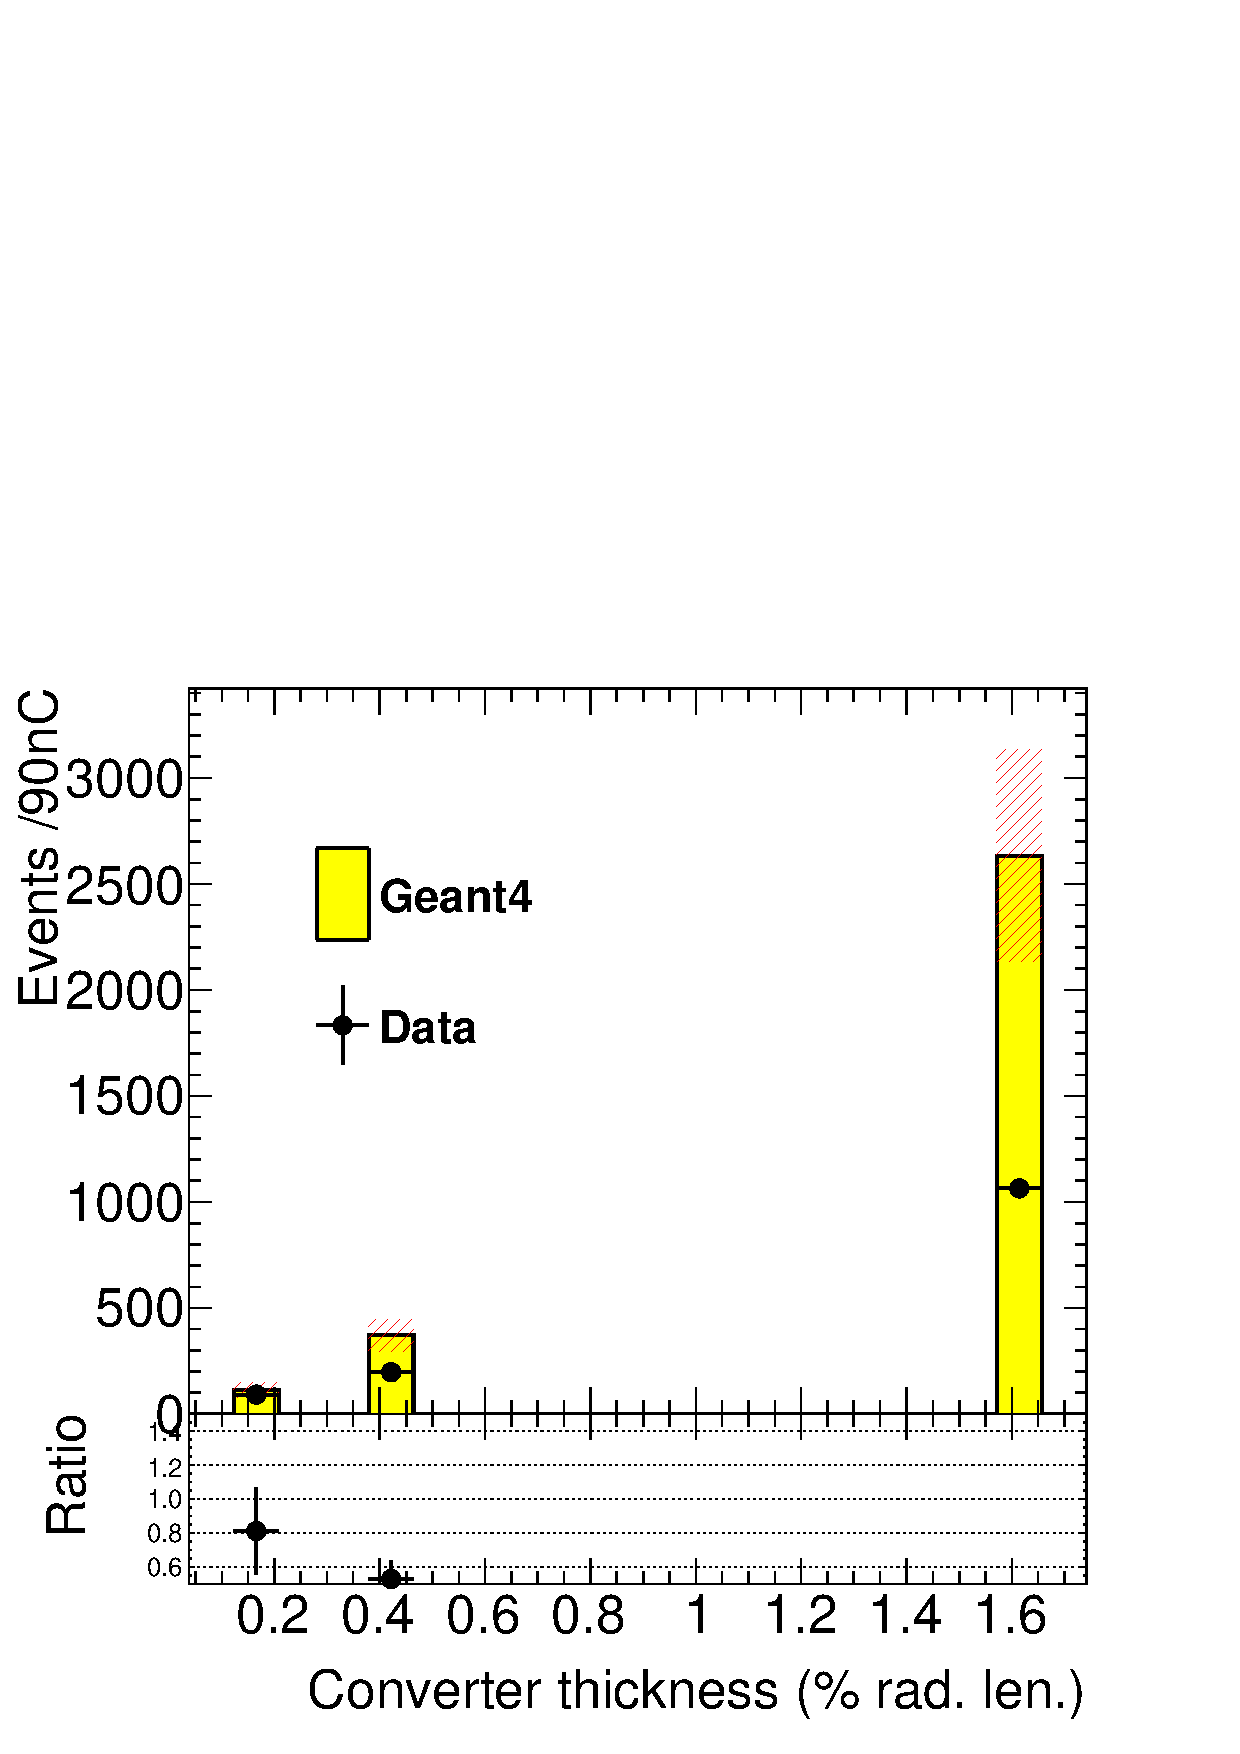
\includegraphics[ scale=0.3]{test2012/angular_measurement/pictures/dataMC_geant4.png}
\includegraphics[ scale=0.3]{test2012/angular_measurement/pictures/dataMC_egs.png}
\caption{\small{The measured rate in the ECal as a function of target thickness comparing 
to the multiple scattering models from {\sc Geant4} (left) and {\sc EGS5} (right)}.} 
\label{fig:ang_distr_data}
\end{figure*}
A few systematic uncertainties was estimated which include; a 5\% uncertainty on the integrated 
current normalization, limited Monte Carlo statistics, alignment of the ECal and uncertainty 
from the background normalization. The uncertainty from the initial gain calibration of the 
ECal described in Sec.{\color{red} X} was estimated to be less than {\color{red} Y\%, need to check this calibration 
systematic.}.

\begin{table}
\begin{tabular}{|l|c|c|c|}
Converter (\% r.l.) & 1.60\% & 0.45\% &	0.18\% \\
\hline
{\sc EGS5} &	1162 $\pm$ 112 &	255 $\pm$ 28 &	94 $\pm$ 17	\\
\hline
{\sc Geant4} & 2633 $\pm$ 250 & 	371 $\pm$ 38 &	114 $\pm$ 18 \\
\hline
Observed 	& 1064 $\pm$ 2 & 196 $\pm$ 1 &	92 $\pm$ 1 \\						
%Beam gap	58	13	5	132	19	6
%	EGS			G4		
%Target thickness	1.60%	0.45%	0.18%	1.60%	0.45%	0.18%
%Data [/90nC]	1064	196	92	1064	196	92
%Pred. [/90nC]	1162	255	94	2633	371	114
%Total uncertainty	112	28	17	250	38	18
%Stat	2	1	1	2	1	1
%						
%Stat MC	11	3	1	16	3	1
%Bkg norm.	14	14	14	14	14	14
%Current norm.	94	21	8	212	30	9
%Beam gap	58	13	5	132	19	6
\hline
\end{tabular}
\caption{ {\small Observed and predicted events for 1~s of beam at 90nA for different converter 
thicknesses. The uncertainty on the predictions is the total uncertainty including estimated 
systematic uncertainties. }{\color{red} Cross-check numbers}}
\end{table}
With the set of conservative systematics the total systematic uncertainty was 
between 10 and 18\%. 

In summary it's clear that the version of  
{\sc Geant4} with the default physics lists overestimates the large angle multiple scattering tail. 
This preliminary result further strengthens our confidence that {\sc EGS5} describes the multiple scattering in the target which is important to understand our expected occupancy and trigger 
rates for HPS. As a side note, since {\sc EGS5} was used to generate the pair 
angle distribution for both simulation described in the result it's interesting to see that the 
ratio of data to that the prediction varied from 0.91 (0.40), 0.77 (0.53) and 0.98 (0.81) for {\sc EGS} ({\sc Geant4}) at 1.6\%, 0.45\% and 0.18\% converter thickness, respectively. If the pair angle distribution were responsible 
for the difference between {\sc Geant4}  and {\sc EGS5} that would show up as a large shift in 
this ratio since the multiple scattering contribution varies. 

There are many steps needed to go from this preliminary result to a real 
measurement. However, this preliminary result further strengthens our confidence that 
{\sc EGS5} is able to properly describe the large angle multiple scattering events in the target 
which is important to estimate our occupancy and trigger rates for HPS discussed in Sec.~\ref{sec:performance}.





